\documentclass[a4paper,11pt]{article}

\usepackage[utf8]{inputenc} % Unicode support (Umlauts etc.)
\usepackage[ngerman]{babel} % Change hyphenation rules
\usepackage{ziffer} % , können in Zahlen verwendet werden ohne Formatierung kaputt zu machen
\usepackage[top=30mm,right=20mm,bottom=15mm,left=25mm,includefoot,headheight=32pt]{geometry} % Seitenränder

\usepackage{lmodern,textcomp} % The package supports the Text Companion fonts, which provide many text symbols (benötigt für €)
\usepackage[fleqn]{amsmath} % Formatierte Gleichungen
\usepackage{graphicx} % Grafiken
\usepackage{xcolor} % Farbe in Text
\usepackage{fancyhdr} % Seitenstil mit Kopfzeile etc.

\usepackage{cases} % Fallunterscheidungen mathematisch uebereinander

\usepackage{floatflt}

\pagestyle{fancy}
\fancyhf{}
\lhead{
    Lösung \\
    Übungsblatt 7
}
\rhead{Gruppe 3 \\Nils \textbf{Hodys}, Sascha \textbf{Majewsky}}
\rfoot{Seite \thepage}

\setlength{\parindent}{0cm} % Keine Einrückung der 1. Zeile eines Absatzes

\begin{document}

\raggedright % Alles Linksbündig

\section{Aufgabe 1}

\subsection*{Entscheidungsvariablen:}
\begin{tabular}{rll}
  $X_{EP}$ &= einfache Platinen & \\
  $X_{KP}$ &= komplexe Platinen & \\
  
  $Y_{A}$ &=\left\{ \begin{array} {l@{\quad}l}1 & \text{Standort A wird gebaut}\\0 & \text{Standort A wird nicht gebaut}\end{array} \right\\
  
  $Y_{B}$ &=\left\{ \begin{array} {l@{\quad}l}1 & \text{Standort B wird gebaut}\\0 & \text{Standort B wird nicht gebaut}\end{array} \right\\
  
  $max~z$ &$= X_{EP} + X_{KP}$\\

\end{tabular}

\subsection{Kapazitätsrestriktionen Standort A:}\
\begin{tabular}{rcrlll}
$X_{EP} &+ &X_{KP}$&\le ~$73.125 &+~M_a(1-Y_a)$ & \text{Produktionskapazität Schmelze pro Woche}\
$X_{EP} &+ &X_{KP}$&\le ~$48.875 &+~M_a(1-Y_a)$ & \text{Produktionskapazität Löten pro Woche }\
$X_{EP} &+ &X_{KP}$&\le ~$66.500 &+~M_a(1-Y_a)$ & \text{Qualitätssicherungskapazitäten pro Woche}\
$0,31X_{EP} &+ &0,24X_{KP}$&\le ~$6500 &+~M_a(1-Y_a)$ & \text{Verfügbarkeit Kupfer pro Woche}\
$0,12X_{EP} &+ &0,12X_{KP}$&\le ~$3900 &+~M_a(1-Y_a)$ & \text{Verfügbarkeit Plastikplatinen pro Woche}\
$0,015X_{EP} &+ &0,025X_{KP}$&\le ~$2600 &+~M_a(1-Y_a)$ & \text{Verfügbarkeit Wolfram pro Woche}\
$0,03X_{EP} &+ &0,02X_{KP}$&\le ~$5900 &+~M_a(1-Y_a)$ & \text{Verfügbarkeit Stahl pro Woche}\
&&$0,055X_{KP}$&\le ~$550 &+~M_a(1-Y_a)$ & \text{Verfügbarkeit Seltene Erden pro Woche}\
\end{tabular}

\subsection{Kapazitätsrestriktionen Standort B:}\
\begin{tabular}{rcrlll}
$X_{EP} &+ &X_{KP}$&\le ~$95.625 &+~M_b(1-Y_{B})$ & \text{Produktionskapazität Schmelze pro Woche}\
$X_{EP} &+ &X_{KP}$&\le ~$60.375 &+~M_b(1-Y_{B})$ & \text{Produktionskapazität Löten pro Woche}\
$X_{EP} &+ &X_{KP}$&\le ~$85.500 &+~M_b(1-Y_{B})$ & \text{Qualitätssicherungskapazitäten pro Woche}\
$0,31X_{EP} &+ &0,24X_{KP}$&\le ~$5700 &+~M_b(1-Y_{B})$ & \text{Verfügbarkeit Kupfer pro Woche}\
$0,12X_{EP} &+ &0,12X_{KP}$&\le ~$3200 &+~M_b(1-Y_{B})$ & \text{Verfügbarkeit Plastikplatinen pro Woche}\
$0,015X_{EP} &+ &0,025X_{KP}$&\le ~$1900 &+~M_b(1-Y_{B})$ & \text{Verfügbarkeit Wolfram pro Woche}\
$0,03X_{EP} &+ &0,02X_{KP}$&\le ~$5100 &+~M_b(1-Y_{B})$ & \text{Verfügbarkeit Stahl pro Woche}\
&&$0,055X_{KP}$&\le ~$410 &+~M_b(1-Y_{B})$ & \text{Verfügbarkeit Seltene Erden pro Woche}\
\end{tabular}

\subsection*{weitere Restriktionen:}
\begin{tabular}{llll}
$X_{EP}$&&\ge ~$1025 & \text{Mindestanzahl Palette einfache Platinen}\\
&$X_{KP}$&\ge ~$1025 & \text{Mindestanzahl Palette komplexe Platinen}\\
$X_{EP}$,&$X_{KP}$ &\ge ~0\\
&$Y_a$, Y_{B}$ &= ~1\\
&$Y_a$, Y_{B}$ &\in \{$1,0$\}


\end{tabular}

\section*{Aufgabe 2}

\subsection*{Definition}
$x_{d}$: Produktionsmenge Fahrrad Deluxe in Stück pro Woche \\
$x_{n}$: Produktionsmenge Fahrrad Normal in Stück pro Woche \\

Bestimmung $z_{1}^{ Opt} = 78000$ via Solver \\
Bestimmung $z_{2}^{ Opt} = 7000$ via Solver \\
Umformung: \\
min $z_{2} = 30x_{d} +20x_{n}$ \\
max $z_{2}^{'} = -30x_{d} -20x_{n}$ \\
Daher gilt $z_{2}^{ 'Opt} = -7000$ \\
\vspace{4mm}
Solver: \\

\begin{centering}
	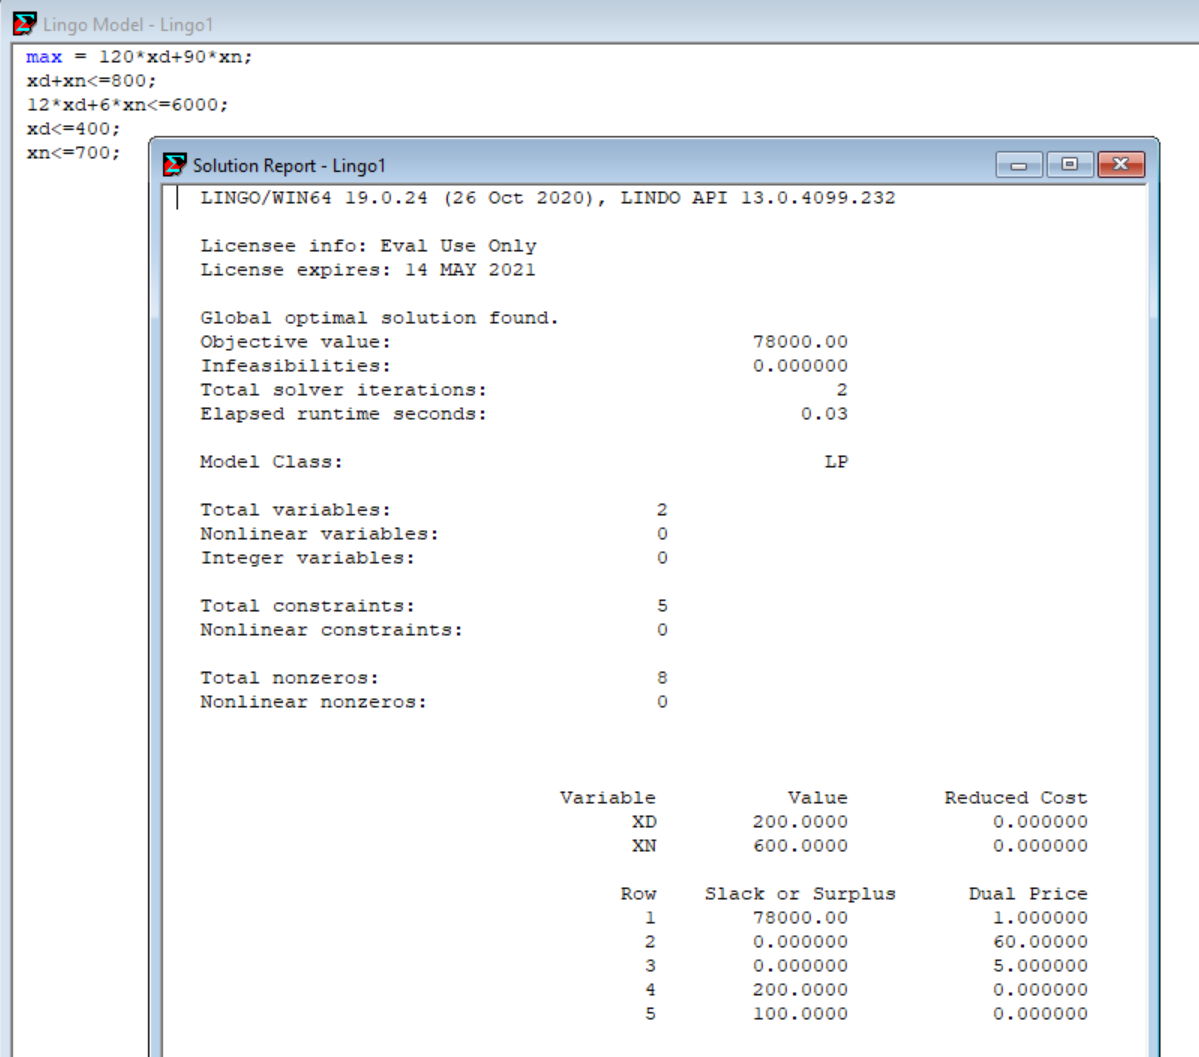
\includegraphics[width=0.65\linewidth]{src/blatt_7_aufgabe_2_solverloesung_1.png}
\end{centering}

\begin{centering}
	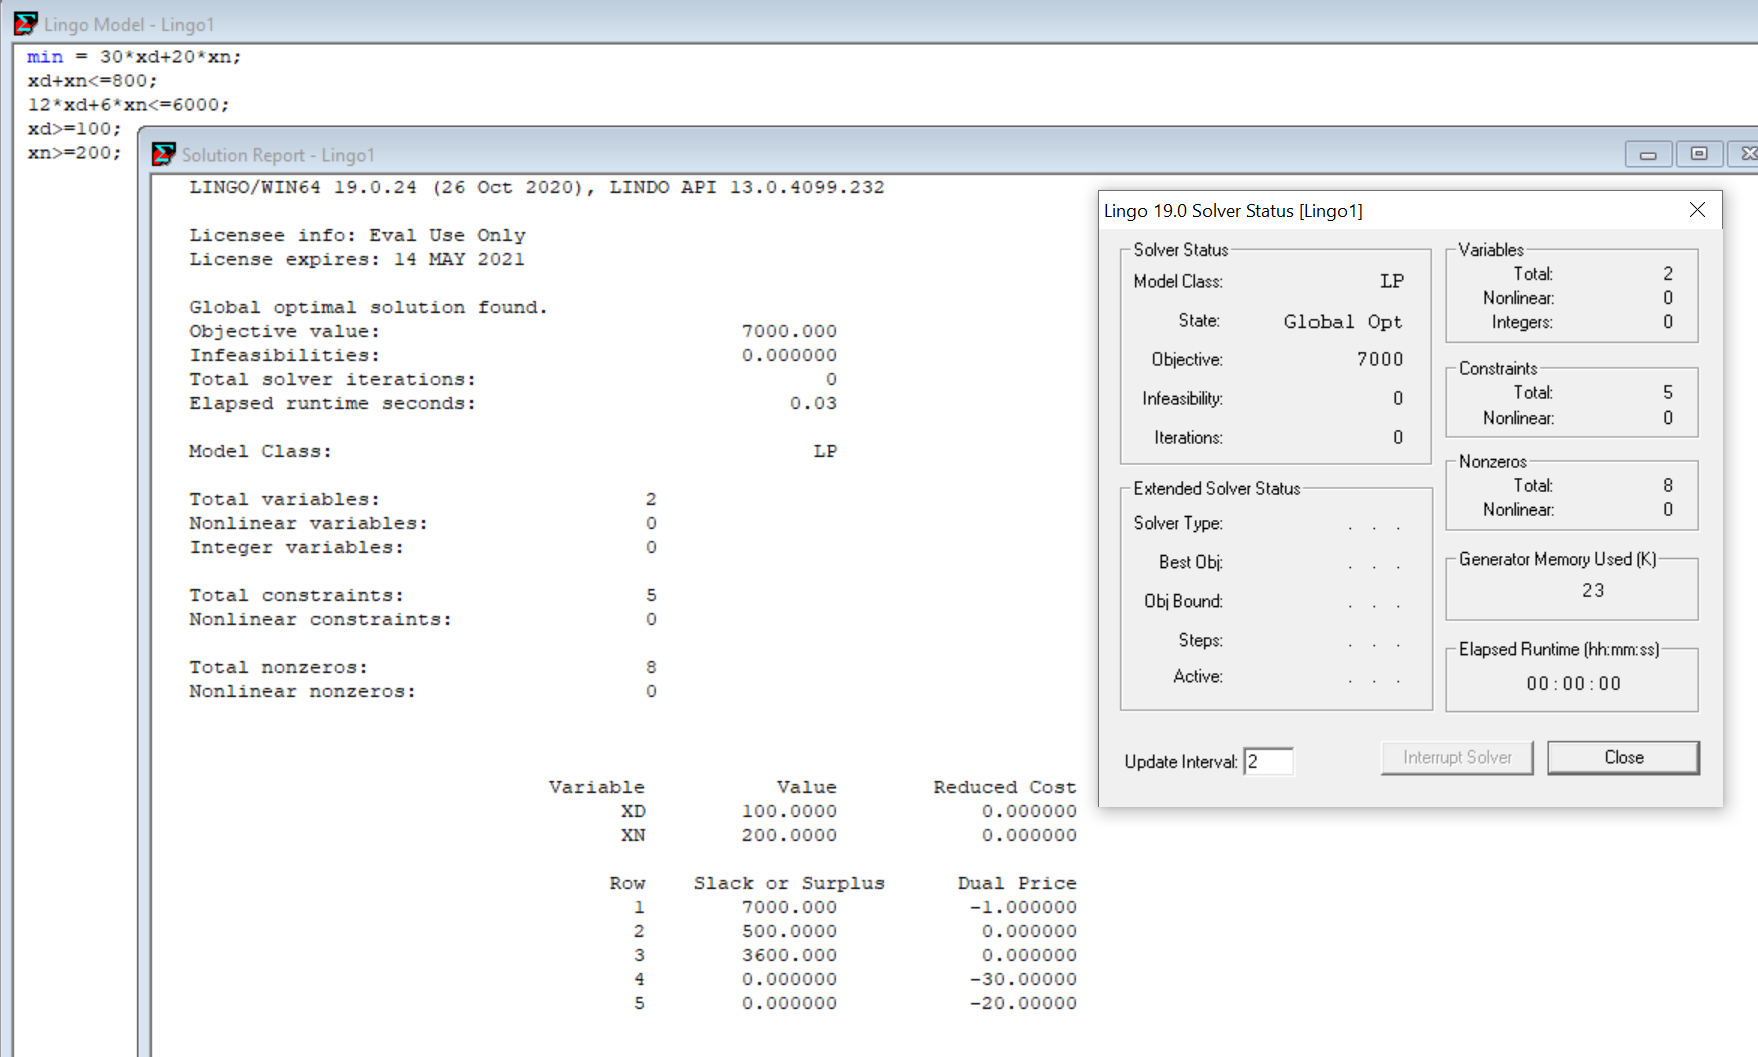
\includegraphics[width=0.65\linewidth]{src/blatt_7_aufgabe_2_solverloesung_2.png}
\end{centering}

\pagebreak
Modellaufstellung: \\

\begin{align*}
    \text{min } &z \\
    \text{s.t. } & x_{d} + x_{n} \le 800 && \text{Max. Produktionsmenge} \\
    & 12x_{d} + 6x_{n} \le 6000 && \text{Max. verfügbare Zeit} \\
    & -30x_{d} -20 * x_{n} + v_{1} = -7000 && \text{Einsetzen $z_{2}^{'}$ mit $z_{2}^{'Opt}$ } \\
    & 120x_{d} + 90 * x_{n} + v_{2} = 78000 && \text{Einsetzen $z_{1}$ mit $z_{1}^{Opt}$ } \\
    & x_{d} \le 400 && \text{Max Anzahl Deluxe pro Woche} \\
    & x_{n} \le 700 && \text{Max Anzahl Normal pro Woche} \\
    & x_{d} \ge 100 && \text{Min Anzahl Deluxe pro Woche} \\
    & x_{n} \ge 200 && \text{Min Anzahl Normal pro Woche} \\
    & v_{1} \le z && \text{} \\
    & v_{2} \le z && \text{} \\
    & x_{d}, x_{n} \ge 0 && \text{Es kann keine negative Menge produziert werden} \\
\end{align*}

Solver: \\

\begin{centering}
	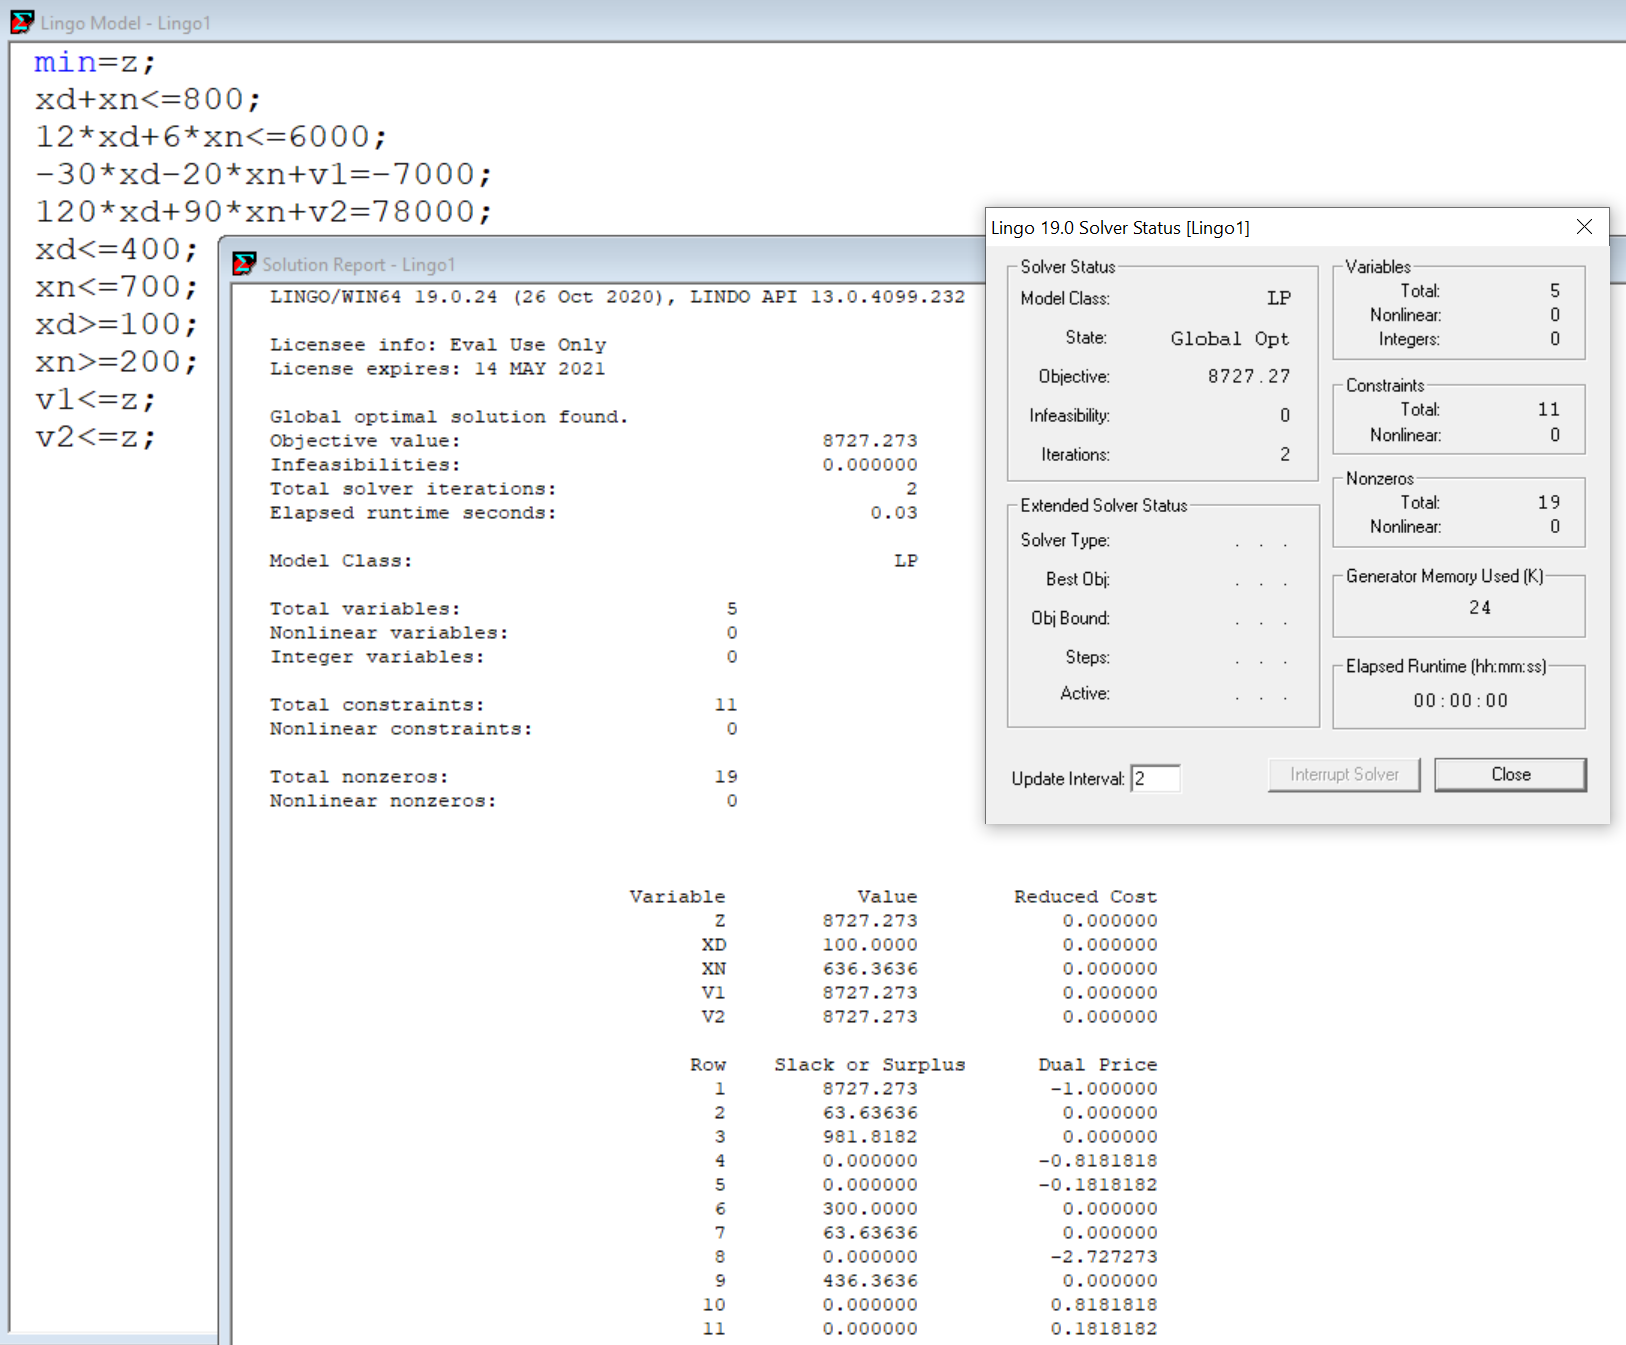
\includegraphics[width=0.65\linewidth]{src/blatt_7_aufgabe_2_solverloesung_3.png}
\end{centering}

\end{document}